% !TeX program = xelatex
\documentclass{ctexart}
\usepackage[table]{xcolor}
\usepackage{template_by_mny}
\usepackage{float} 
\usepackage{listings}
\lstset{basicstyle=\ttfamily, breaklines=true, frame=single}

\title{光谱仪教学实验报告}
\class{物理 32/物理 31}
\name{冯家琦/周方远}
\id{2023011338/2023011263}

\begin{document}
\maketitle

\begin{abstract}
本实验使用EDU-SPEBCT1扩展光谱仪教学套件,完成了绿光波长测量、样品吸收率光谱图等实验。通过实验加深了对光谱仪工作原理的理解,掌握了光谱测量的进阶方法。
\end{abstract}

\section{实验原理}

反射光栅光谱仪是一种用于分析光谱的光学仪器。其基本原理包括:
\begin{figure}[H]
    \centering
    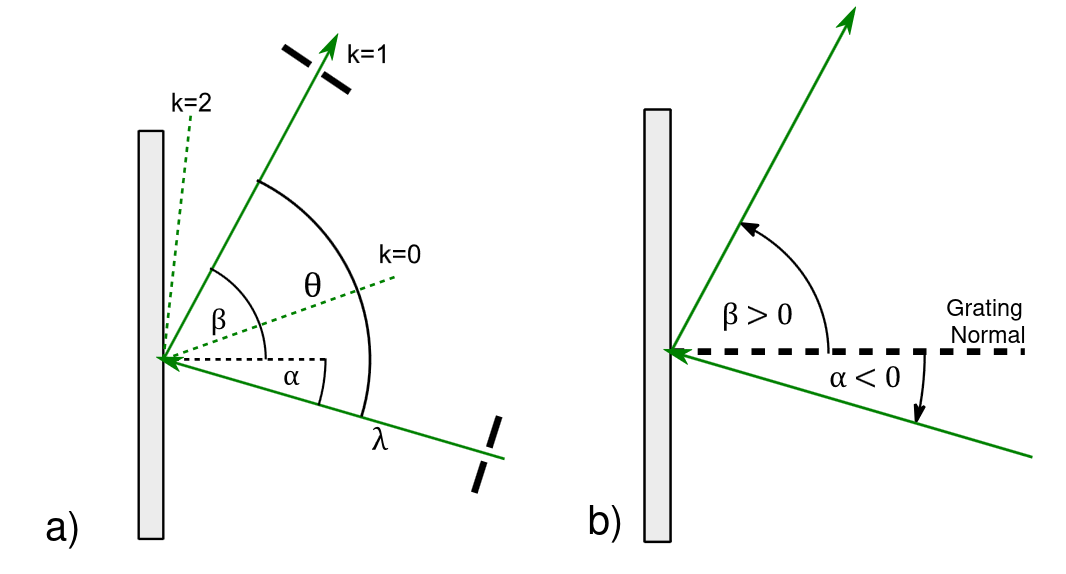
\includegraphics[width=0.6\textwidth,height=0.3\textwidth]{pictures/原理图例.png}
    \caption{衍射角与入射角和级数的关系}
\end{figure}

如图所示,k 表示衍射级数,$\lambda$ 是波长,$\alpha,\beta$ 分别是入射角和出射角,d 为光栅间距。它们满足如下关系:
\[k\cdot\lambda=\sin\beta\cdot d+\sin\alpha\cdot d\]
\subsection{光谱仪的组成}
一个基本的光谱仪包含以下部件:
\begin{itemize}
    \item 入射狭缝:控制入射光束宽度
    \item 反射聚焦镜:将光线聚焦到光栅上
    \item 分光元件:反射光栅
    \item 聚焦系统:再用凹面镜将分光后的光聚焦
    \item 观测屏/探测器:用于观测光谱
\end{itemize}

\section{实验仪器及安装}
\subsection{实验仪器}
\begin{itemize}
    \item EDU-SPEB2光谱仪教学套件
    \item 可调节狭缝
    \item 三棱镜
    \item LED光源及其USB供电支架
    \item 双凸透镜(f=50mm和100mm)
    \item 观测屏
    \item 其他光学元件支架和固定件
\end{itemize}
\subsection{仪器安装}


\section{实验步骤}
\subsection{确定波长}
根据以下公式可计算波长
\begin{align}
    \theta &= -2 \alpha_{cal} \\
    \lambda &= \frac{\sin(\theta+\alpha)+\sin(\alpha)}{g}
\end{align}
代入数据得到
\begin{align}
    \theta &= 55.166 \\
    \lambda &= \frac{\sin(55.166-17.166)+\sin(-17.166)}{600} = 534.2nm
\end{align}
测量数据及计算结果如下
\begin{table}[h]
    \centering
    \begin{tabular}{|c|c|c|c|}
        \hline
        \rowcolor{yellow!25} Spectral Line & Wavelength [nm] (Literature)  & Angle of Incidence $\alpha$ (Measured) & Wavelength [nm] (Calculated)   \\
        \hline
        Zero Order Reflection & \- & -27.583 & \-  \\
        \hline
        Bandpass Filter & 532 & -17.166 & 534  \\
        \hline
    \end{tabular}
\end{table}
\subsection{参考光谱}
\begin{itemize}
    \item 逆时针旋转 PR01(/M)旋转台的千分尺螺钉,直到读取到清晰的数值。
    小心地逆时针旋转 PR01(/M) 旋转台的千分尺螺杆,直到可以在 PR01(/M) 的游标刻度上读出一个清晰的数值。
    记录平台的旋转角度和万用表上的信号。
    \item 通过 PR01(/M) 的逆时针运动将平台旋转一个固定的步长。
    并记录每一步的角度和万用表信号,直至微调范围的极限值。
    测微螺杆仍会转动,但平台不会转动。
    关闭光源,记录万用表的信号值。
    记录万用表的信号值。 稍后将从数据中减去背景光
\end{itemize}
经过以上步骤,得到数据
\begin{table}[!ht]
    \centering
    \begin{tabular}{|l|l|l|l|l|l|l|l|l|l|l|l|l|l|l|l|l|l|l|l|l|l|l|l|l|l|l|l|l|l|l|l|l|l|}
    \hline
        背景光(mV) & 0.62 & ~ & ~ & ~ & ~ & ~ & ~ & ~ & ~ & ~ & ~ & ~ & ~ & ~ & ~ & ~ & ~ & ~ & ~ & ~ & ~ & ~ & ~ & ~ & ~ & ~ & ~ & ~ & ~ & ~ & ~ & ~ \\ \hline
        波长(nm) & 340 & 340.25 & 340.5 & 340.75 & 341 & 341.25 & 341.5 & 341.75 & 342 & 342.25 & 342.5 & 342.75 & 343 & 343.25 & 343.5 & 343.75 & 344 & 344.25 & 344.5 & 344.75 & 345 & 345.25 & 345.5 & 345.75 & 346 & 346.25 & 346.5 & 346.75 & 347 & 347.25 & 347.5 & 347.75 & 348 \\ \hline
        光强(mV) & 0.73 & 0.84 & 1.68 & 4.63 & 10 & 6.26 & 3.55 & 3.08 & 4.89 & 7.8 & 10.74 & 13.11 & 15.29 & 16.69 & 17.7 & 18.44 & 17.5 & 13.79 & 11.3 & 9.83 & 8.39 & 7.15 & 5.99 & 4.96 & 3.53 & 2.94 & 2.44 & 2.05 & 1.77 & 1.5 & 1.29 & 1.16 & 1.04 \\ \hline
    \end{tabular}
\end{table}
\begin{figure}[H]
    \centering
    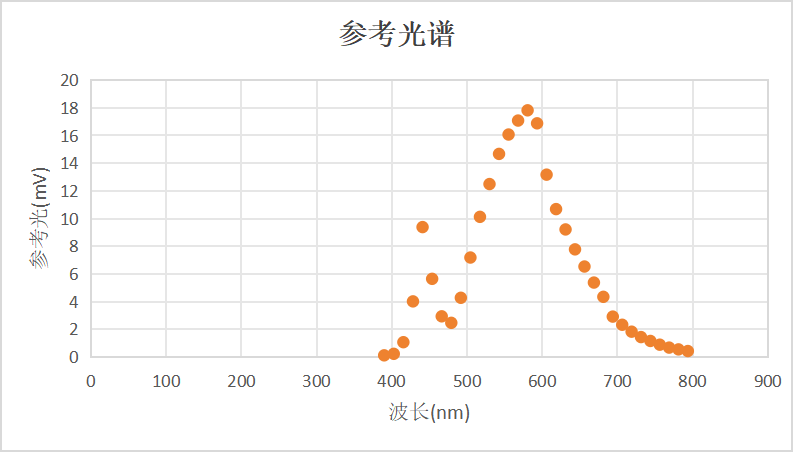
\includegraphics[width=0.8\textwidth]{pictures/图片1.png}
    \caption{参考光谱}
\end{figure}

\subsection{样品光谱}
往透镜后加入样品,搭建光路如图
\begin{figure}
    \centering
    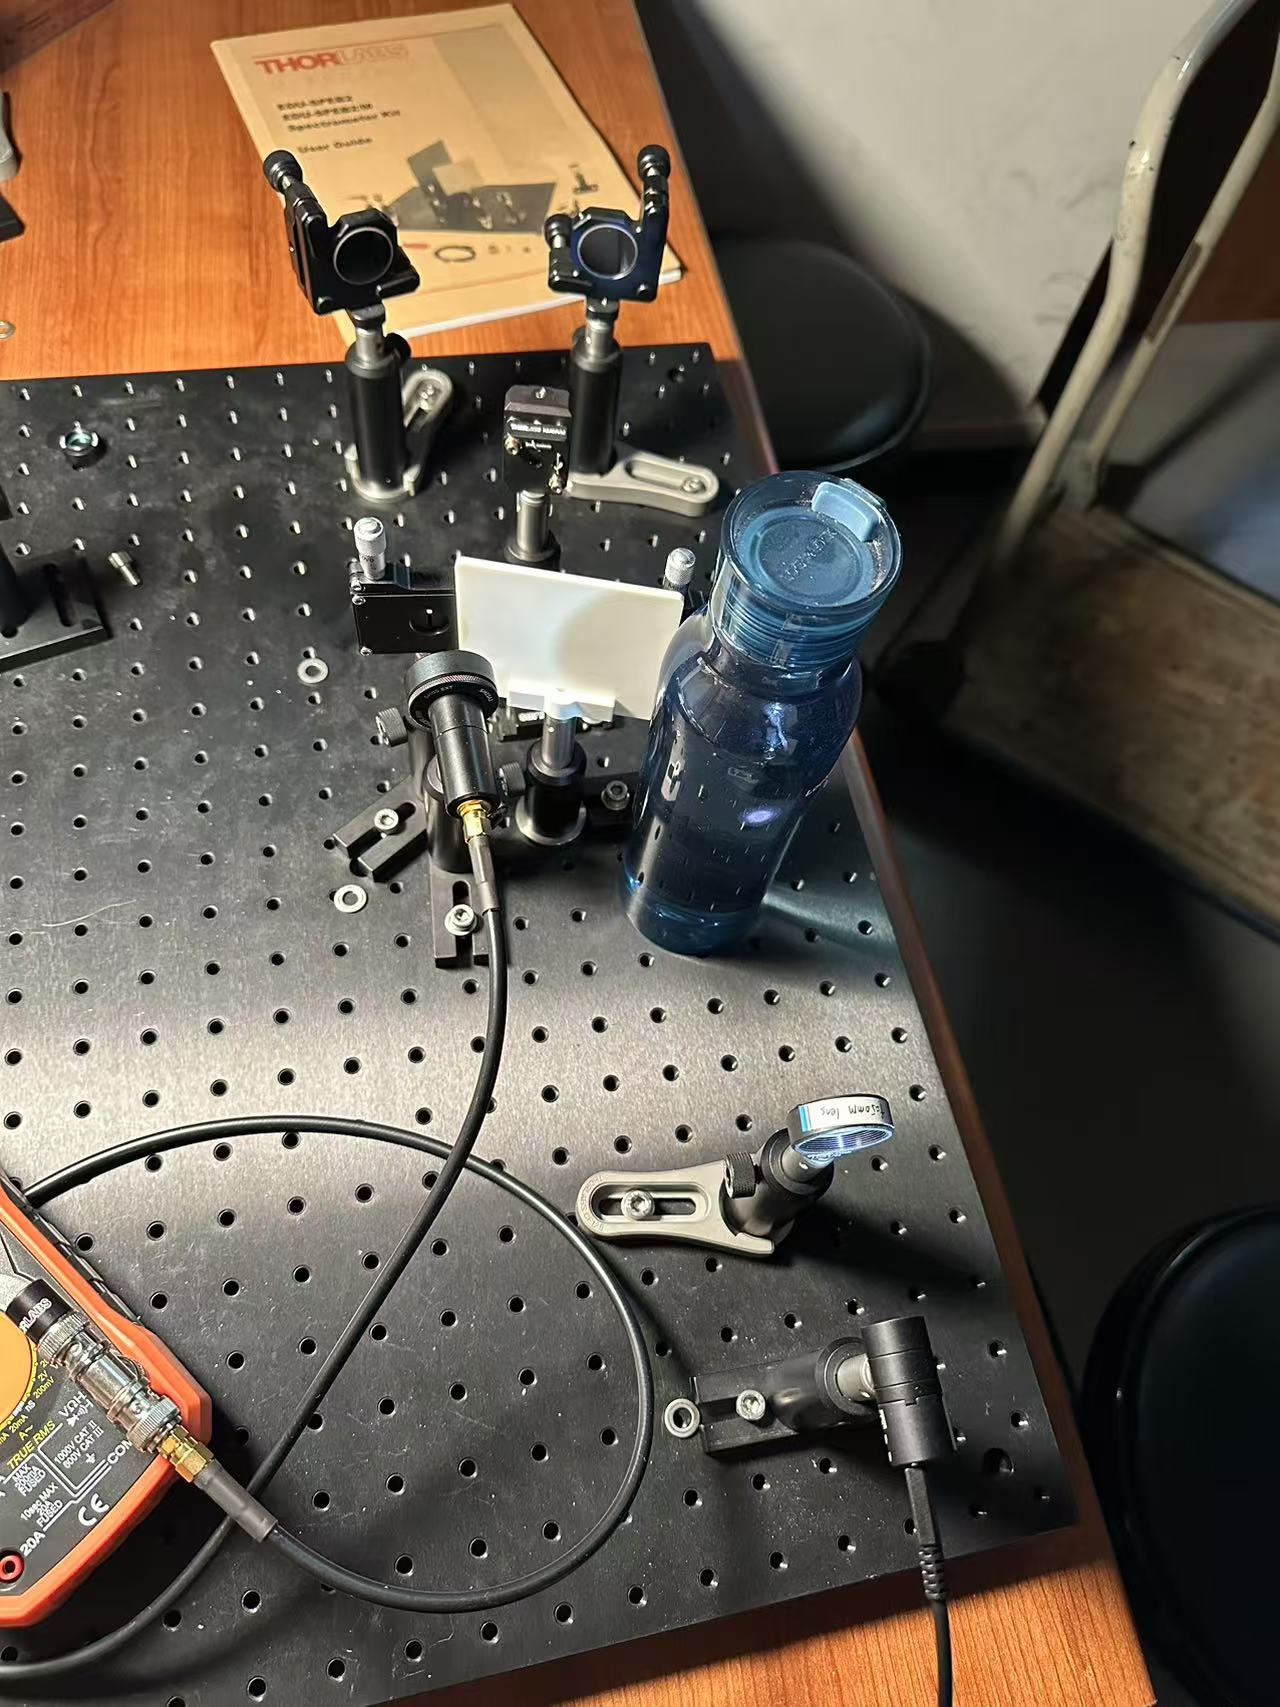
\includegraphics[width=0.4\textwidth]{pictures/微信图片_20241121154954.jpg}
    \caption{光路}
\end{figure}

重复以上步骤,测量得到
\begin{figure}[H]
    \centering
    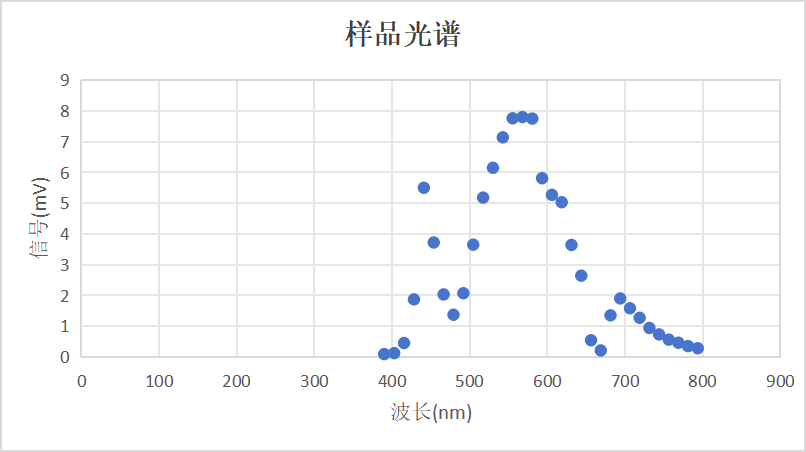
\includegraphics[width=0.8\textwidth]{pictures/图片2.png}
    \caption{样品光谱}
\end{figure}

\subsection{数据分析:吸收谱线}
将相同波长处的样品光强与参考光强相除,得到吸收率,并以波长为横坐标,吸收率为纵坐标绘制吸收谱线
\begin{figure}[H]
    \centering
    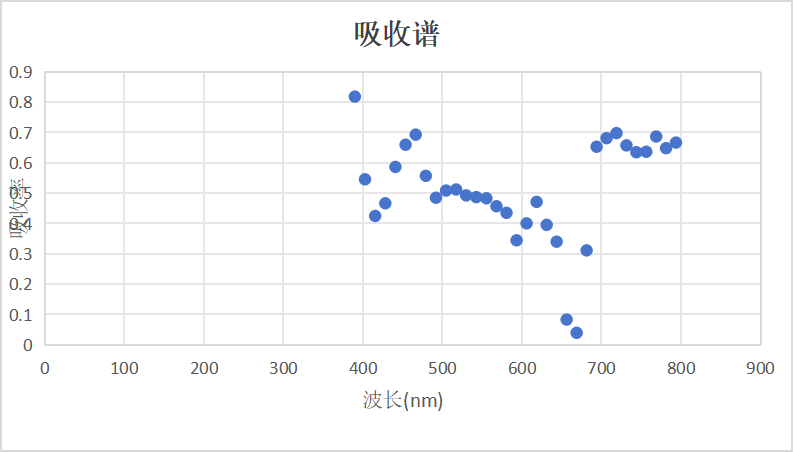
\includegraphics[width=0.8\textwidth]{pictures/图片3.png}
    \caption{吸收谱线}
\end{figure}

\section{实验思考}

\section{总结}
**

\end{document}